\documentclass[phd,tocprelim]{thesis}
%% Added to avoid the \ifpdf name clash error
\let\ifpdf\relax
%
% tocprelim option must be included to put the roman numeral pages in the
% table of contents
%
% The cornellheadings option will make headings completely consistent with
% guidelines.
%
% This sample document was originally provided by Blake Jacquot, and
% fixed up by Andrew Myers.
%
%Some possible packages to include
\usepackage{graphicx,pstricks}
\usepackage{graphics}
\usepackage{moreverb}
\usepackage{subfigure}
\usepackage{epsfig}
\usepackage{subfigure}
\usepackage{hangcaption}
\usepackage{txfonts}
\usepackage{palatino}
\usepackage[graphicx]{realboxes}


\usepackage{graphicx}
\usepackage{import}
\usepackage{wrapfig}
\usepackage{hyperref}
\usepackage{amssymb}
\usepackage{amsmath}
\usepackage{tikz}
\usepackage{xfrac}
\usepackage{tabu}
\usepackage{color}
\usepackage{cite}
\usepackage{array}
\usepackage{listings}
\usepackage{parskip}
\usepackage{nicefrac}
\usepackage{listings}
\usepackage{fancyhdr}
\usepackage{enumitem}
\usepackage{multirow}
\usepackage{tocloft}
\usepackage{float}
\usepackage{array}
\usepackage{subfig}
\usepackage{gensymb}
\usepackage{multicol}
\usepackage{subfig}
\usepackage{pdfpages}
\usepackage{url}

\usepackage[pdftex]{graphicx}
\usepackage{float}
\usepackage{booktabs,caption,fixltx2e}


%if you're having problems with overfull boxes, you may need to increase
%the tolerance to 9999
\tolerance=9999

\bibliographystyle{plain}
%\bibliographystyle{IEEEbib}

\renewcommand{\caption}[1]{\singlespacing\hangcaption{#1}\normalspacing}
\renewcommand{\topfraction}{0.85}
\renewcommand{\textfraction}{0.1}
\renewcommand{\floatpagefraction}{0.75}

\title {Mapping and Classification of Microorganism}
\author {Emilie M Hyrum Dahl}
\conferraldate {December}{2018}
\degreefield {MSc}
\copyrightholder{Emilie M Hyrum Dahl}
\copyrightyear{2018}

\begin{document}
%Veldig viktig med konsistens i table of contents. Feks kan vi ha sånn at alle forbokstaver på alle ord er stor..

\maketitle
\makecopyright

\begin{abstract}
The ocean plays a great part in life on earth, not only as a source to oxygen and food for living beings, but also as a vital influence to the climate and weather. The ocean, with all that comes with it, is simply a necessity for life on earth. Nevertheless, this same ocean is not taken care of. Millions of pieces of plastics, especially micro-plastic, pollutes and eradicate sea life every day, indirectly affecting life on land. 
\\\\
The road to a clean sea can be divided into steps. First step is to prevent the continuous supply of trash and plastic pollution. The next step should involve picking up what is already in the ocean. The latter action is further divided into sub-steps. As ocean is huge, attacking all parts of the sea is next to impossible. Being able to map and monitor the ocean columns and determine critical areas is thus a good start. Therefore, this thesis will concern methods for detection and analyzing micro-plastics. 

%An abstract is a brief summary of a research article, thesis, review, conference proceeding, or any in-depth analysis of a particular subject and is often used to help the reader quickly ascertain the paper's purpose.
\end{abstract}

\begin{preface}
This thesis is submitted in partial fulfillment of the requirements for the degree of master of science (MSc) at the Norwegian University of Science and Technology (NTNU). The main work is conducted at Department of Marine Technology, NTNU, while part of the work has been conducted at the Department of Biology, NTNU in cooperation with Aksel Mogstad. 
\\\\
I have cooperated with Andreas Stien in large part. Next to all testing and work done hands on, have been done together with Andreas. Therefore we share the same approach and results. 

\end{preface}

\begin{acknowledgements}
This project thesis and final report has been supported by members of the faculty at NTNU. The author of this report would particularly like to thank supervisor Professor Asgeir J. Sørensen at IMT NTNU and PhD. candidate Aksel Mogstad, who have been at close guidance throughout this project and the entire semester. 
\\\\
In addition, a great thanks should be directed towards Professor Geir Johnsen at the Department of Biology NTNU, who provided insight and expertise that greatly assisted the project and thereby this report.
\end{acknowledgements}

\begin{summary}
Your summary goes here. Make sure it sits inside
the brackets.
\end{summary}

\contentspage
\tablelistpage
\figurelistpage

\normalspacing \setcounter{page}{1} \pagenumbering{arabic}
\pagestyle{thesis} \addtolength{\parskip}{0.5\baselineskip}

\chapter{Introduction}
\section{Motivation}
%and Background??

%The background of the study will discuss your problem statement, rationale, and research questions. It links introduction to your research topic and ensures a logical flow of ideas.  Thus, it helps readers understand your reasons for conducting the study.
%HER MÅ JEG OGSÅ HA MED AT SOM NEVNT I ABSTRACT, MÅ VI GJENNOM FLERE STEG. NESTE STEG ER Å DESIGNE EN SENSORBÆRENDE PLATFORM SOM KAN BRUKE DETEKSJONSMETODENE. 

%http://ec.europa.eu/environment/marine/good-environmental-status/descriptor-10/pdf/GESAMP_microplastics%20full%20study.pdf

Today, the applications for plastics are huge, making the material popular worldwide. %335 million metric tons of plastic was produced in 2016. %(https://www.statista.com/statistics/282732/global-production-of-plastics-since-1950/)
% https://www.darrinqualman.com/global-plastics-production/
Approximately 400 million metric tons of plastic is produced yearly, and the production is projected to nearly double within the next 10-15 years. %https://wedocs.unep.org/bitstream/handle/20.500.11822/25398/WED%20Messaging%20Two-Page%2027April.pdf?sequence=12&isAllowed=y
In addition to being a strong, light and inexpensive material, the different types of plastic cover an almost full-scaled spread of needs. High electrical isolation properties are useful in one area, while durable and strong material can be ideal in other areas. What do we read of this? Plastics have incredibly useful and versatile properties. However, this worldwide spread of plastics holds a significant side effect. 

The different types of plastic have polymer structures that make the material almost non-biodegradable. In addition, the structures of plastics can hold additives. This is initially something that can be utilized, as additives can be incorporated in order to give the plastic a desired property. Typically additives are fire retardants, stabilizers, antibiotics, pigments etc. %[https://www.darrinqualman.com/global-plastics-production/]
Problems arise when the additives that blend into the pieces of plastics, turns out to be toxins and the plastic debris serves as a vector, introducing toxic elements into the ecosystem. As this vector is not biodegradable, it can travel between ecosystems as an immortal catalyst.

The largest source of microplastic is the discharge of larger plastic pieces gradually fragmented into smaller plastic debris. The fragmentation occurs due to wear and tear from the environment. The biggest cause of decomposition is UV radiation from the sun. The rays provide oxidative decomposition of polymers, which in turn will give weak and brittle plastic debris. At this state, mechanical forces can easily fragment the weak plastic piece. Of such forces wind, waves and human activity are good examples. The state of a large plastic piece floating around the many seas can thereby quickly result in many smaller pieces and in turn be fragmented to microplastic.

%The interesting thing here is the adding of additives that stabilize for example UV radiation, and thereby reducing the rate of fragmentation and the amount of microplastic. Of course, this will not change the fact that the original plastic piece floats around, but this is still a better result from an environmental point of view.

%https://setac.onlinelibrary.wiley.com/doi/10.1002/ieam.5630030412
The largest issue with microplastic is due to ingestion by marine biota. Once microplastic is ingested, it is in most cases retained in the digestive system or absorbed by the intestines. After a while, the plastic debris are stored in organs and tissue. Due to the fact that plastics are not biodegradable, the chemicals will hardly be excreted by the organism ingesting the piece, but rather accumulate. This is called bioaccumulation. 
\\\\
%https://www.sciencedirect.com/science/article/pii/S0160412017322298 
Bioaccumulation creates the foundation of biomagnification, causing the poisoning of entire food chains. Organisms and animals placed at a higher trophic level are often in need of a larger amount of food than what the species on a lower level can serve. This consumption need means that the concentrated bioaccumulation is even larger at higher trophic levels. In fact, the concentration of an environmental toxicity increases with each level of the food chain - in turn affecting human beings as well. This is called biomagnification. 
\\\\
An example of a typical bioaccumulated chemical, traveling through trophic levels, is Polychlorinated biphenyls (PCBs), a group of manmade chemicals. Ryan et al. (1988) proved that PCB in the bird's tissue originates from plastic particles.(*) Sadly PCBs are harmful chemicals, even in very low amounts. The ingestion of PCB can cause reproductive disorders, change the hormone levels and increase the risk of several diseases. In some cases, an intake can lead to death [(Ryan et al., 1988, Lee et al., 2001)].
\\\\
Furthermore, different types of bacteria are attracted to free floating marine debris. These are better known as “hitch hikers”, and can threaten sensitive coastal environments, as the bacteria are far from their natural habitats. 
%(Environmental implications of plastic debris in marine settings-entanglement, ingestion, smothering, hangers-on, hitch-hiking and alien invasions Murray R. Gregory)
Some phytoplankton eating species are particularly exposed, as microplastic easily can be confused with phytoplankton. One of the most common types of microplastic, polystyrene (PS), has shown to affect the ability to reproduce. %(http://www.pnas.org/content/113/9/2430).
\\\\
Different types of plastic have different densities. Some types have higher density than water and float, while other types are denser than water. This contributes to the fact that plastic can be found throughout the entire ocean column, and is present in many ecosystems(*). As a result, plastic debris have impacted more than 690 marine. Small particles of plastic have been observed in the digestive tract of organisms from different trophic levels. 
\\\\
While microplastics does damages as a toxic carrying vector, larger pieces of plastics can act as a physical threat in other ways. Polyethylene bags, operating in the ocean currents, have a large resemblance to the predators targeted by turtles. (*) Plastic debris can thus prevent their survival (Bugoni et al., 2001, Duguy et al., 1998). The ingestion of larger plastic debris can, among other things, reduce food intake, cause internal damage, strangling or even death after blockage of the intestinal tract. (Zitko and Hanlon, 1991).
\\\\
Marine biological diversity is already exposed to climate change, over-fishing and other man-made disruptions. As if this were not enough, plastic pollution, with more than 8 billion kilograms entering the ocean annually
%[http://www3.weforum.org/docs/WEF_The_New_Plastics_Economy.pdf],
also causes huge damage to the marine environment. (*)
%* = The pollution of the marine environment by plastic debris: a review Jose G.B. Derraik *

\subsection{Taking Action}
Now that the large impact of plastic is clear, methods on how to reduce this impact are in order. A good way to work with materials, identify them or learn about their properties, is to study how light interacts with them - spectroscopy. By definition spectroscopy examines how light behaves in the target and recognizes materials based on their different spectral signatures. This can be identified from the spectrum, describing the amount of light in different wavelengths, showing how much light is reflected, emitted and transmitted from the target. In other words, the spectrum simply shows how much of a certain color the light contains. 
\\\\
Spectral signatures can be thought of as fingerprints. While fingerprints often is used to identify a person, spectral signatures can be used to identify materials. One of the purposes of this study, is to identify different types of plastic using their spectral signatures. %A thought: As different types of plastic are composed by different polymer structure accepting additives in various degree, one might be able to identify the plastic types most resistant to additives

%Development of hyperspectral imaging as a bio-optical taxonomic tool for pigmented marine organisms - geir
Former studies conducted on marine organisms, show that reflectance signatures, obtained from an underwater hyperspectral imager, are related to the absorption signature of that specific organism. %(Volent et al. 2007, 2009)
\\\\
The research questions driving this project are centered around whether microplastics and their spectral signatures in fact can be separated from other material and microorganisms. Do different types of plastics leave different spectral signatures? Could a signature change as the sea tears the plastic pieces? Is it possible that the spectral signatures differ in different environments?

\section{Research Question}
The latter questions are important to address when detecting and inspecting microplastic in the ocean. This thesis will dive deeper into some of these questions, in particularly one question; Do different types of plastics obtain different spectral signatures within visual light?

\section{Main Contributions} This paragraph is currently a placeholder. In this section the breaking results will be described in short (elevator pitch). This result could be why [result] is in particularly suitable when detecting microplastic.
\\
(If moving passed the spectra of visual light, the wavelengths are too large to penetrate the water as wanted. When the waves propagate with a very high frequency, the light cannot go through water as desired. Therefore, the visual light spectra is a constraint when looking at the resulting signatures). NO, we cannot separate the different types of plastic based on their spectral signature. However, when testing with other organisms, a clear clustering is presented. The challenge is that in order to classify the plastics, the rest of the material or organisms in the image needs to be classified - (method of elimination). 

\section{Thesis Outline}
%denne kan vel være i preface eller noe?
The work supporting this thesis is three-folded. In order to achieve relevant and precise knowledge, a literature study was conducted. This study involved research on both specific methods and technology used, and what has been done in general. The research regarding these topics were done mainly through reading scientific papers. However, even with the most recent publications, there are still research done - not yet published. The second part of this thesis was therefore to travel around Trondheim meeting with the experts. During exciting meetings with Emlyn, Andy, Geir, Aksel, Bert, Asgeir, Atle and Albert (from now on referred to as "the experts"), new knowledge was acquired. After this, the problem description finally took form. Through planning with the experts, the experiment description were formed. These experiments represent the third and last part of the three-folded work. 

%Hva alle kapittelene handler om

\begin{figure}
  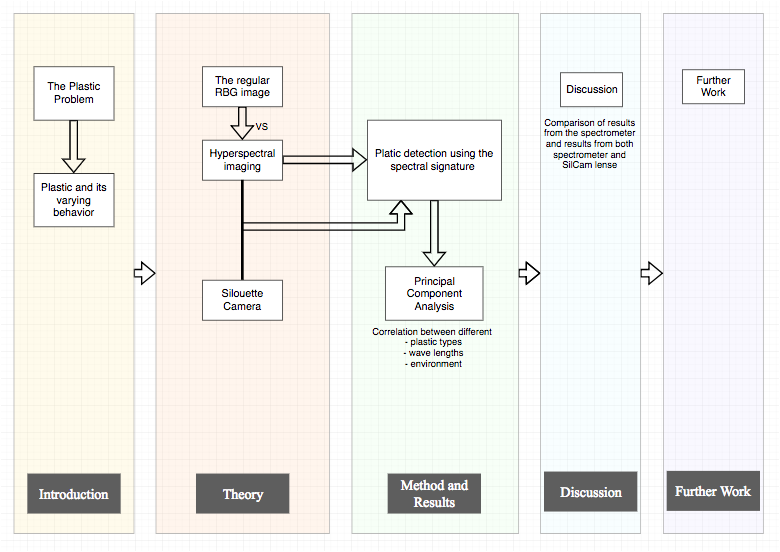
\includegraphics[width=\linewidth]{Images/outline.png}
  \caption{Thesis Outline, roughly sketched}
  \label{fig:outline}
\end{figure}



\chapter{The Problem}
\section{Plastics}
\todo[inline]{vurderer å ha hele/deler av seksjonen om plast fra background her}

\begin{comment}
Marine biological diversity is already exposed to climate change, overfishing and other man-made disruptions. As if this were not enough, plastic pollution also causes huge damage to the marine environment. (*)
\\
335 million metric tons of plastic was produced in 2016. %(https://www.statista.com/statistics/282732/global-production-of-plastics-since-1950/)
It is projected that the production will nearly double within the next 10-15 years
%https://wedocs.unep.org/bitstream/handle/20.500.11822/25398/WED%20Messaging%20Two-Page%2027April.pdf?sequence=12&isAllowed=y
\\\\
%Plastic polymers commonly found in the environment are polypropylene (PP), polyethylene (PE), polyethylene terephthalate (PET), polystyrene (PS) and polyvinylchloride (PVC).8 Together these comprise 72.9 percent of the plastic produced globally.9
Kanehiro et al. (1995) states that plastic accounted for 80-85 percent of the seabed waste in Tokyo Bay in the 90's. (*)
This is a striking finding, considering that most plastic residues are floating to some degree. Different types of plastic have different densities. Some types have higher density than water and float, while other types are denser than water. This contributes to the fact that plastic can be found throughout the sea column, and is present in many ecosystems. For instance, plastics have been found in the digestive system of organisms of all sizes, from small marine invertebrates to whales.
\\\\
Polyethylene bags, operating in the ocean currents, have a large resemblance to the predators targeted by turtles. (*) Plastic debris can thus prevent their survival (Bugoni et al., 2001, Duguy et al., 1998). The ingestion of plastic debris can, among other things, reduce food intake, cause internal damage, strangling (hvordan bøyes dette) or even death after blockage of the intestinal tract. (Zitko and Hanlon, 1991).
\\\\
Plastic is also a potential carrier of chemicals and can absorb bacteria already present in the ocean, including polychlorinated biphenyls (PCBs). (*) PCBs are harmful chemicals, even in very low amounts. The ingestion of PCB can cause reproductive disorders, change the hormone levels and increase the risk of several diseases. In some cases, an intake may lead to death [(Ryan et al., 1988, Lee et al., 2001)]. Ryan et al. (1988) proved that PCB in the bird's tissue originates from plastic particles. Plastic pellets can thus be transporter for PCB in marine food chains (Mato et al., 2001).
\\\\
Furthermore, different types of bacteria are attracted to free floating marine debris. These are better known as “hitch hikers”, and can threaten sensitive coastal environments, as the bacteria are far from their natural habitats. 
%(Environmental implications of plastic debris in marine settings-entanglement, ingestion, smothering, hangers-on, hitch-hiking and alien invasions Murray R. Gregory)
\\\\
Some phytoplankton eating species are particularly exposed, as microplastic easily can be confused with phytoplankton. One of the most common types of microplastics, polystyrene (PS), has shown to affect the ability to reproduce %(http://www.pnas.org/content/113/9/2430).
%* = The pollution of the marine environment by plastic debris: a review Jose G.B. Derraik *
\end{comment}

\section{Today}
Solving today’s plastic problem is not an easy task - especially when plastic and microplastic are not only present in the water surface, but in the entire water column. Imagine multiplying the entire ocean surface with a few hundred meters dept. This leaves an almost impossible starting point. In addition, there are continuous currents and motion, allowing a large spread. On top of it all, the deep sea is difficult to reach, and if reaching it, poor sight is often a fact. So, what have been done so far in order to solve this plastic problem?
\\\\
The problem with plastic is becoming an increasingly known problem. Since plastic contamination and many of its consequences are visible to the naked eye, few people can deny that the pollution of plastic is a fact. Nevertheless, it is not enough to be aware of the problem – the world must cooperate and act. Today there are solutions like ocean cleanup, etc\todo{mer av dette}. The challenge with these solutions is that they do not necessarily go towards high concentrated areas. Today we know that large pieces of plastic travel to the garbage patch ....\todo{og dette} (Evidence that the Great Pacific Garbage Patch is rapidly accumulating plastic 2018, L. Lebreton1,2, B. Slat1, F. Ferrari1 – mer herfra). Nevertheless, the entire ocean needs to be mapped.
\\\\
One obvious requirement when mapping and cleaning the ocean of plastic, is the availability of an instrument able to detect plastic in the ocean separating it from the rest of the ocean particles. This is where the field of spectroscopy enters the court. The development of image detectors, especially the two-dimensional silicon charge coupled device (CCD), has revolutionized image spectroscopy. CDD provides information on the distribution of photon intensity along the spectrograph's entrance slit. The distribution of entrance slit into different wavelengths and intensities, has made it possible to reconstruct detailed images at high spatial (defined as 1 cm) and spectral (defines as 1 nm) resolution. This makes a hyperspectral imager particularly suitable, as it consists of a spectrometer equipped with this charge coupled device (CCD). 
% (Development of hyperspectral imaging as a bio-optical taxonomic tool for pigmented marine organisms - geir)

%(BASIC HYPER SPECTRAL IMAGING F. SIGERNES)
%G. Vane, ed., Imaging Spectroscopy II, Proc. SPIE 834, 1988.
%W.L. Wolfe, Introduction to Imaging Spectrometers, Vol. TT25 of Tutorial Text Series, SPIE Press, Bellingham, Wash., pp. 1-147, 1997.
The last decade, most of the work and discovery in hyperspectral imaging, have been within space and air-born sensors. Here, the instrument has proven to be a particularly powerful remote control tool. It is not until recently that the technology has been tested underwater. As the sea is not stagnant and objects in water can behave differently than in air, new challenges can occur. Nevertheless, research shows that the technology is promising, also underwater, and can be a very useful tool when detecting microorganisms.
\\\\
In addition, work on detection and classification of plastic in the sea, has been conducted, using hyperspectral imaging underwater. \todo{mer fra bert sitt arbeid}
%Bert: http://journals.sagepub.com/doi/pdf/10.1255/jnirs.1212 (mer herfra). 
\\\\
Furthermore, the Silhouette camera (SilCam) developed by SINTEF, is also interesting in this matter. This technology is different, as it utilizes a light source behind the object to be identified to clearly see the outline of the target. Simplified, the hyperspectral imagery extracts the contents of what is depicted, while the SilCam captures the exterior. The question is, can these two methods compliment each other and give an even better way of detecting micro-organisms? This has never been tried before.
\todo[inline]{skrive sånn at avslutningen her blir mer oppgavepresis}

Experiments analyzing the wave spectra of different types of plastics, have already been conducted. However, the results has been directed towards viewing the wave length interval describing near infrared light (NIR). Although the use of infrared light is an effective means of unobtrusive observation on land, it is far less effective in the ocean because long wavelength light is rapidly attenuated by seawater.

PAPER: Identification and Classification of Plastic Resins using Near Infrared Reflectance PSpectroscopy: https://www.researchgate.net/publication/285330830_Identification_and_classification_of_plastic_resins_using_near_infrared_reflectance_spectroscopy

%https://oceanoptics.com/plastic-recycling-nir-spectroscopy/ Plastic Recycling with NIR Spectroscopy - denne inneholder signaturene til plast i NIR
Another important observation in these experiments, is the condition of the microplastic used. The material is pure and white, making the results independent of color. 

Water absorption 
%https://commons.wikimedia.org/wiki/File:Absorption_spectrum_of_liquid_water.png
This logarithmic (log-log) graph shows water’s absorption behavior at different colors wavelength. As seen in the graph, water absorption is minimised between 400 -600 nm


Light Transmission in the Ocean: http://www.waterencyclopedia.com/La-Mi/Light-Transmission-in-the-Ocean.html
https://manoa.hawaii.edu/exploringourfluidearth/physical/ocean-depths/light-ocean



\chapter{Theory}
%- Hva karakterieserer plast utifra hva vi vet
%- ulike sensorer for deteksjon og kartlegging (vise sammenhengen til dette og en bredere oversikt - dette blir isåfall bare her, men tas ikke med videre - i metode kan vi heller si at vi avgrenser mot cam)
%- aktuelle sensorer 
%- sensorbærende plattform
%- PCA og singular value Decomp

%(alt dette kan evt komme kort i motivasjon) 


\section{Light}
%Color Registration of Underwater Images for Underwater Sensing with Consideration of Light Attenuation
%https://ieeexplore.ieee.org/stamp/stamp.jsp?tp=&arnumber=4209801
Light is electromagnetic radiation. The human eye can detect electromagnetic radiation within wavelengths of 400 and 750 nm, approximately. This electromagnetic spectrum is called visible light. Radiation with shorter wavelength than 400 nm is called ultraviolet, whereas infrared radiation has longer wavelength than visible light.

When light from a light source hits an object surface, the light is reflected before eventually reaching the eye. In this task, the endpoint will not only be the human eye, but other viewpoints, for instance a camera lens. The observation of the reflected colors in the viewpoint, is affected by properties of object surfaces, the light intensity of light source and traveling distance of the light.

Light in air behaves differently than in water. In air, the light will not be attenuated, which means that the reflection can be expressed by the light intensity, $I_ {\lambda}$ (eq \ref{eq:int}), describing the colors observed on the object.

\begin{equation} \label{eq:int}
    I_ {\lambda} (L, z) = \frac{S \cdot \kappa_{\lambda}\cdot cos^{3}\cdot (\alpha)}{z^2}
\end{equation}


In equation \ref{eq:int}, $I_{\lambda}$ represents the light intensity at a given wavelength, lambda, while S is the light source. L is the distance between the object and the viewpoint, while z describes the distance from the object to the light source. Furthermore, $\kappa_{\lambda}$ describes the reflectance ratio of the object's surface at a given wavelength, $\lambda$. $\alpha$ is the angle between the ray vector from the light source and the normal vector of the object surface.


\begin{figure}[H]
\centering
  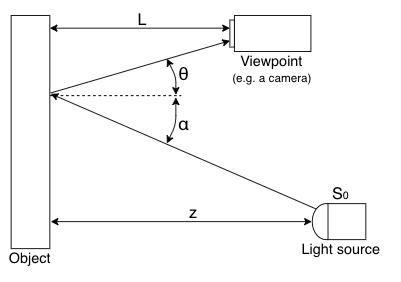
\includegraphics[width=12cm]{Images/theory/reflectance.png}
  \caption{Light refraction in liquid}
  \label{fig:reflectance}
\end{figure}



However, it is different if we do the same underwater. In water, light attenuation will be present and affect how the light is reflected.

\section{The Behavior of Light in Water}

%The light intensity decreases with the distance from objects in water by light attenuation depending on the wavelength of light. Red light decreases easier than blue light in water [E. O. Hulburt: “Optics of Distilled and Natural Water,” Journal of the Optical Society of America, Vol.35, pp.689–705, 1945].

The reason why the color of objects is different under water and in air, is that the light intensity, in water, decreases with the distance (r) to the object. This is, as mentioned, due to light attenuation, which again depends on the wavelength of the light. %([E. O. Hulburt: “Optics of Distilled and Natural Water,” Journal of the Optical Society of America, Vol.35, pp.689–705, 1945].) 
\\\\
From figure \ref{fig:lightinwater}, it can be observed that the intensity of the different colors decreases differently, even at the same distance, r. If the light source is 2 m away, red light will shine at half intensity, while blue light remains close to unchanged. At a distance of 20 meters, blue light will brighten at half-intensity. In this case, red and orange color will disappear.
%Color Registration of Underwater Images for Underwater Sensing with Consideration of Light Attenuation
%https://ieeexplore.ieee.org/stamp/stamp.jsp?tp=&arnumber=4209801

\begin{figure}[H]
\centering
  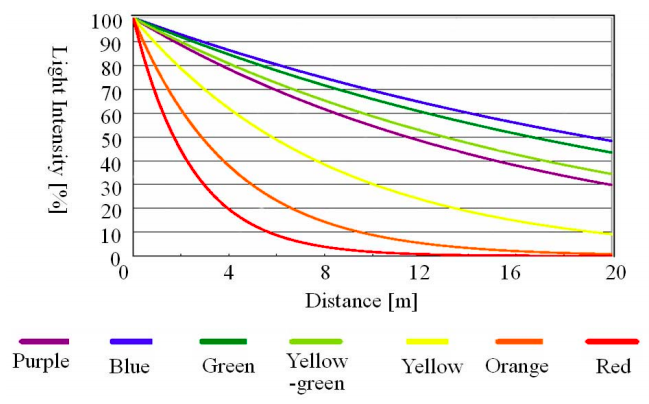
\includegraphics[width=12cm]{Images/theory/intensity.png}
  \caption{Light intensity in water.}
  \label{fig:lightinwater}
\end{figure}

As shown in the figure \ref{fig:lightinwater}, the light intensity decreases exponentially. The figure, is based on the following equation for the light source, S. 

\begin{equation} \label{eq:source}
S_{\lambda} (z) = S_0 \cdot exp (-c_{\lambda} \cdot r)
\end{equation}

In eq \ref{eq:source}, $S_{\lambda}$ describes the light intensity at wavelength $\lambda$, while $S_0$ is the intensity at the light source. Furthermore, r describes the distance between the light source and the viewpoint, while $c_{\lambda}$ is the attenuation coefficient of the wavelength $\lambda$, illustrated by figure \ref{fig:attcoeff}.
\\\\
By taking the attenuation coefficient, $c_{\lambda}$, into consideration, the light intensity in water can be expressed by the following similarity. 

\begin{equation} \label{eq:intw}
    I_ {\lambda} (L, z) = \frac{S \cdot \kappa_{\lambda}\cdot cos^{3}\cdot (\alpha)}{z^2} \cdot exp \left(-c_{\lambda}\left(\frac{z}{cos(\alpha)}\frac{L}{cos(\theta)}\right)\right)
\end{equation}

When interpreting eq \ref{eq:intw}, one can see that the intensity of light decreases when $c_{\lambda}$ increases. If $c_{\lambda} = 0$, meaning the light attenuation not being present, the resulting intensity becomes the same as the light intensity in air, eq \ref{eq:int}. 

\begin{figure}[H]
\centering
  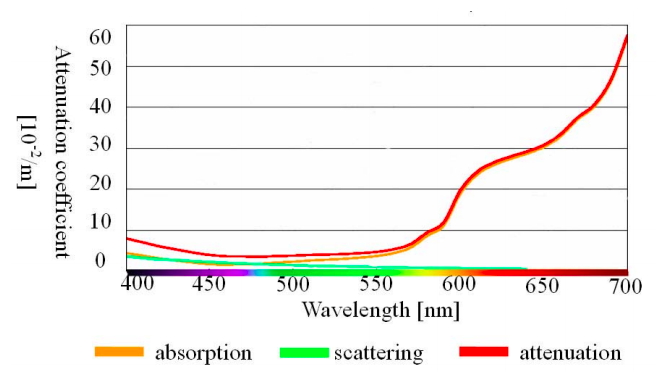
\includegraphics[width=12cm]{Images/theory/attcoeff.png}
  \caption{Attenuation coefficient}
  \label{fig:attcoeff}
\end{figure}


%Attenuation coefficient consists of absorption coefficient and scattering coefficient, because light attenuation consists of light absorption and light scattering. Attenuation coefficient of water changes very much with the wavelength of light. Consequently, observed colors changes in underwater environments.


%Stereo Measurement of Objects in Liquid and Estimation of Refractive Index of Liquid by Using Images of Water Surface
%http://www.robot.t.u-tokyo.ac.jp/~yamashita/paper/B/B047Final.pdf
Note: If cameras and objects are in the different condition where the refraction index differs from each other, several problems occur and a precise measurement cannot be achieved.

\section{Inherent Optical Properties}
%http://iopscience.iop.org/article/10.1088/0034-4885/36/12/002/pdf


%noe av dette har blitt sagt i hyp også:
When retrieving an optical fingerprint it is important to know the optical properties impacting the resulting signature. There are mainly three physical processes reducing the energy of light on its way to reaching the receiver. The object of interest (the materials or the compositions of materials) will absorb, scatter and reflect light of different portions of the visible spectrum. This way, the material of the object of interest and the wavelength will affect the properties of these processes. 

Scattering, absorption and reflection are both a result of photons interacting with the object of interest. 

%http://www.oceanopticsbook.info/view/overview_of_optical_oceanography/inherent_optical_properties
\subsection{Absorption}
During the photon-IOO interaction, the energy of the photon can be converted to another form, leaving the photon to disappear and hence the light to be absorbed. 

%https://www.physicsclassroom.com/class/light/Lesson-2/Light-Absorption,-Reflection,-and-Transmission
Atoms and thereby molecules contain elections. Given the specific atom, these electrons hold a specific natural frequency. Whenever light hits these molecules, the electrons in that molecule will be given a vibrating motion if the frequency of the light is equal to the electrons natural frequency. This vibration is causing energy – energy taken from the lights photons. This way, the electrons absorb the energy of the light by turning it in to vibration energy, which cannot be converted back to light. 

Different atoms will absorb light at different wavelengths, because they hold different sets of natural vibration frequencies. 

\todo[inline]{pluss coeff og internsitets-likn?}
\todo[inline]{pluss figur?}

\subsection{Scattering}
During the photon-IOO interaction, the photon might either change its direction, its energy or both. Either of these processes are called scattering. %http://iopscience.iop.org/article/10.1088/0034-4885/36/12/002/pdf 
More precisely, scattering can be defined as \textit{the change in direction of light flux produced by individual parcels of particulate matter called ‘scatterers’}. This means that light, or other moving particles, are forced to deviate from the straight trajectory they were on to being with, due to the collision between the light wave and the OOI. 

%http://www.oceanopticsbook.info/view/overview_of_optical_oceanography/inherent_optical_properties 
As mentioned, these inherent optical properties are again dependent on many other properties. Different materials absorb and scatter very much differently as a function of wavelength. If comparing to particles with the same volume, they will scatter light differently if are of different shapes. Similarly, particles with exact same shape will scatter light differently whenever the volume of the particles differ. A change in the material, size or shape (or the composition of them) will give different IOPs. 

In the ocean, the physical characteristics of the IOO are highly affected by the surroundings, implying that the IOPs are too. As an example, a change in the concentration of plankton or being in coastal waters instead of the open ocean, will contribute to a significant change in both the resulting absorption and scattering. 


\subsection{Spectral Reflectance}
%SKRIV OM DENNE

%Underwater hyperspectral imaging: a new tool for marine archaeology 2018, ØYVIND ØDEGÅRD,1,2,* AKSEL ALSTAD MOGSTAD,3 GEIR JOHNSEN,3 ASGEIR J. SØRENSEN, AND MARTIN LUDVIGSEN1
Raw data consists of more than upwelling radiance reflected from the object. Reflections from the water column, ambient light and noise sensors are all parts of the data collected. However, the spectral reflectance reference is independent of the illumination and the water column properties. 

%Underwater hyperspectral imagery to create biogeochemical maps of seafloor properties 2013, G. JOHNSEN, NTNU
The spectral reflectance or ‘optical fingerprint’ can be described as a percentage of how much light at each wavelength is reflected off an object. Different objects absorb and reflect different wavelengths. In plants, red and blue wavelengths are highly absorbed, leaving the reflected color to be more or less green. Mathematically speaking, the spectral reflectance, $R(\lambda)$ is upwelling irradiance coming off the object, $Lu(\lambda)$, divided by the spectral downwelling irradiance towards the object, $Ed(\lambda)$.

%The use of underwater hyperspectral imaging deployed on remotely operated vehicles – methods and applications - geir og asgeir
\begin{equation} \label{eq:specref}
    R(\lambda) = \frac{Lu(\lambda)}{Ed(\lambda)}
\end{equation}

Where $Lu(\lambda)$ denotes the raw data of the object, including signature from light source, while $Ed(\lambda)$ is the spectral radiance from measurements of spectrally neutral reflectance standard.

Note: For eq \ref{eq:specref} to hold true, all surfaces are assumed to behave like Lambertian reflectors. 
%The use of underwater hyperspectral imaging deployed on remotely operated vehicles – methods and applications - geir og asgeir


\section{The Digital Image}
%evt Fysikken bak bildet 
%Info hentet fra bok: techniques and applications of hyperspectral image analysis

From the mid-20th century, images have been stored in digital format (Geladi and Grahn, 2000). A digital image is an array of rows (i) and columns (j) consistent of i x j gray-values. A gray-value, better known as an intensity or a pixel, is simply one of many small squares in an image. If the image is to consist of colors however, a third dimension is needed. This dimension is shown as the depth in FIGURE.. The depth is three intensities/layers deep, consisting of red, green and blue. What was previously a gray pixel is now a voxel, a triplet of red, green and blue.
\\\\
One can say that a color image has three layers, red, green and blue, each of which contains different information. However, if the interval separating the layers is chosen to be a shorter wavelength, the number of layers will increase. The resulting image is then called a multivariate image. If k denote the depth dimension and thus determine the number of wavelengths which in turn will constitute the number of layers, the resulting array will be of the size i x j x k. FIGURE!
\\\\
For a human eye to be able to perceive a color image, only three wavelengths / layers are needed, namely red, green and blue. It therefore rarely makes sense to create multiple layers unless the goal is to capture information the eye cannot see. This is where hyperspectral imaging enters the playing field, which by definition has more than 100 layers and can express each pixel as a spectrum.

\begin{figure}[H]
  \newcommand*\FigVSkip{0.5em}
  \newcommand*\FigHSkip{0.1em}
  \newsavebox\FigBox
  \centering
  % Top image is centered, so no need to get width
 \sbox{\FigBox}{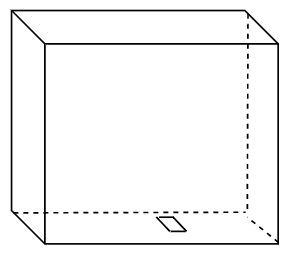
\includegraphics[scale=0.5]{Images/theory/pixel.png}}
  \begin{minipage}{\wd\FigBox}
    \centering\usebox{\FigBox}
    \subcaption{a) Pixel}
  \end{minipage}
  % Save first image in a box to get the width
  \sbox{\FigBox}{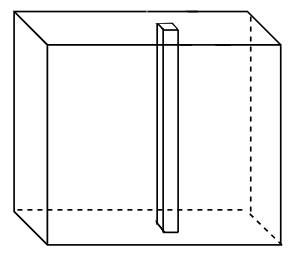
\includegraphics[scale=0.5]{Images/theory/voxel.png}}
  \begin{minipage}{\wd\FigBox}
    \centering\usebox{\FigBox}
    \subcaption{b) Voxel}
  \end{minipage}\hspace*{\FigHSkip}
  % Save second image 
  \label{head}
\end{figure}

\section{Imaging Process}
%Denne skal jeg få tilsendt av Asgeir
???????????


\section{Hyperspectral Imaging}
%Use of Underwater Hyperspectral Imager (UHI) in Marine Archaeology 2014, Øyvind Ødegård1,3, Geir Johnsen2 and Asgeir J. Sørensen1

Hyperspectral imagery is defined as images that contain a spectrum of reflected light with a spectral resolution of 1-5 nm per image pixel (4). Materials or compositions of materials (object of interest, OOI) will absorb, scatter and reflect light of different portions of the visible spectrum, giving them their own optical fingerprints that are unique, and can be used for classification with high degree of confidence (4). 

%Info hentet fra yt
In order to study the reflecting light from the target, a spectrometer is needed. A spectrometer is an instrument that splits the incoming light into a spectrum. Measuring this reflectance spectra is the most common way to use hyperspectral imaging.

\todo[inline]{Masse mer fra modul om hvordan spektrometer fungerer}

\\\\
Hyperspectral imaging uses an imaging spectrometer (also called a hyperspectral camera) to collect spectral information. As mentioned, the difference between a hyperspectral image and a regular photo, is that the hyperspectral camera measures hundreds of thousands of spectra instead of single spectrum, creating a multispectral image. But in contrast to multispectral imagers, which are sensitive in only a few selected wavebands, hyperspectral imagers (HI) measure the spectral upwelling radiance Lu(λ) or reflectance R (λ) per image pixel of bio-geo-chemical object of interest (Klonowski et al. 2007; Volent et al. 2007; Johnsen et al. 2009, 2013b). %(Development of hyperspectral imaging as a bio-optical taxonomic tool for pigmented marine organisms - geir)

This way, the resulting image of the target includes a complete spectrum for each pixel in the image. By doing this, it is possible to extract useful information about the image. 

\\\\
%The spectral information in every pixel creates a third dimension, providing a collection of data called a data cube. Now, how does this data differ from the data and images from other types of cameras? Digital camera, shoots the target in red, green and blue, in order to match the human vision. These camera leaves a combination of the three colors, which is what we can see with our eyes. This means that the information constituting the third dimension consists of nothing more than three colors, while the hyperspectral camera records hundreds of wavelengths. This way, the hyperspectral camera can collect more detailed information about the target, not only in visible light, but also in infrared and ultra violet. By combining different wavelengths, pixel by pixel, one can extract useful information about the properties of the target. 




%Hyperspectral imaging and data analysis for detecting and determining plastic contamination in seawater filtrates, 2016,  Bert van Bavela
%http://journals.sagepub.com/doi/pdf/10.1255/jnirs.1212
Concerning plastics, this translates to receiving information on both spatial location of plastic material, and the plastic materials composition. 
%Volent, Z., Johnsen, G., & Sigernes, F. (2007). Kelp forest mapping by use of airborne hyperspectral imager. Journal of Applied Remote Sensing, 1, 011503–011521.
%Volent, Z., Johnsen, G., & Sigernes, F. (2009). Microscopic hyperspectral imaging used as a bio-optical taxonomic tool for micro- and macroalgae. Applied Optics, 48, 4170–4176.

%(Development of hyperspectral imaging as a bio-optical taxonomic tool for pigmented marine organisms - geir)
HI and UHI can be used as a taxonomical identification tool to make optical fingerprints of marine organisms only if the pigment composition and corresponding absorption signature of the organism is known and can be used to verify the reflectance signature

When the hyperspectral camera is taken underwater, the lighting is limited. The UHI is therefore using its own light sources, in contrast to passive passive techniques using ambient light (Johnsen et al. 2013b).
%(Development of hyperspectral imaging as a bio-optical taxonomic tool for pigmented marine organisms - geir) %The use of underwater hyperspectral imaging deployed on remotely operated vehicles – methods and applications - geir og asgeir


%Info hentet fra bok: techniques and applications of hyperspectral image analysis
 %oppsettene inkluderer lyskilde, et filtersystem som disperse the light into bands of wavelenghts, en sample. Hvis kilden inneholder et bredt lysspekter, kan man velge ut bølgelengder ved å bruke bandpass-filters etter ønske.
\\\\In this task, there are two methods for camera configurations, point scanning image and line scanning image.
\subsection{Point Scanning Image}
Point scanning image can be used to measure a complete spectrum in one spot/pixel. In every spot, all layers are measured vertically from this spot. To make the whole picture, the camera must scan across the entire surface, spot by spot.
\\\\
figuren er hentet fra boken, techniques and applications of hyperspectral image analysis, side 6

% \begin{figure}[H]
%   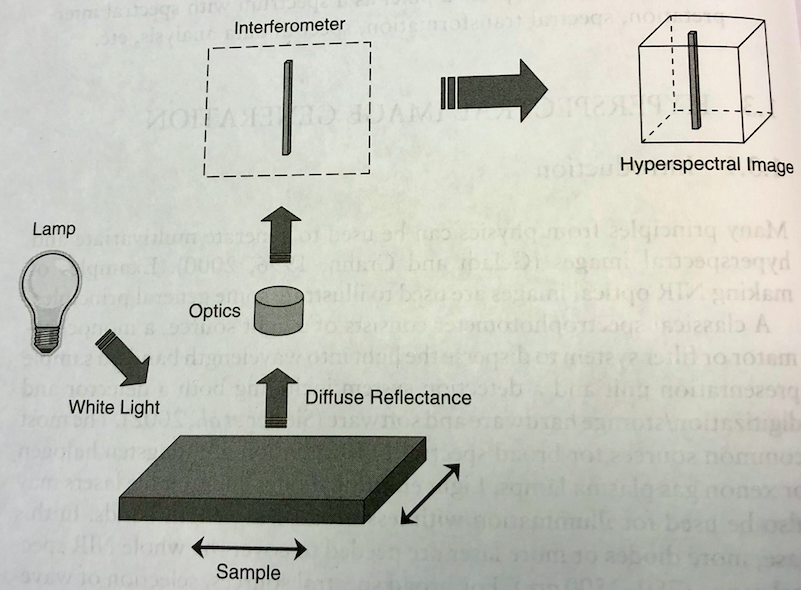
\includegraphics[height=12cm]{Images/theory/pointscan.png}
%   \caption{Set-up, Point Scanning Image}
%   \label{fig:pointscan}
% \end{figure}


\begin{figure}[H]
\centering
  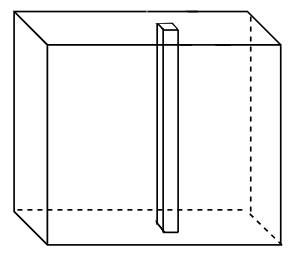
\includegraphics[height=6cm]{Images/theory/voxel.png}
  \caption{Resulting scan}
  \label{fig:voxel2}
\end{figure}


\subsection{Line Scanning Image}
The line scanning image technique uses a two-dimensional detector, perpendicular/orthogonal to the surface of the measured target. This detector collects the spectrum of a whole line in the image, in one single scan. By moving the scan line with a push broom technique, one can map the entire image by combining all sets of spectra.
\\\\
figuren er hentet fra boken, techniques and applications of hyperspectral image analysis, side 7

% \begin{figure}[H]
% \centering
%   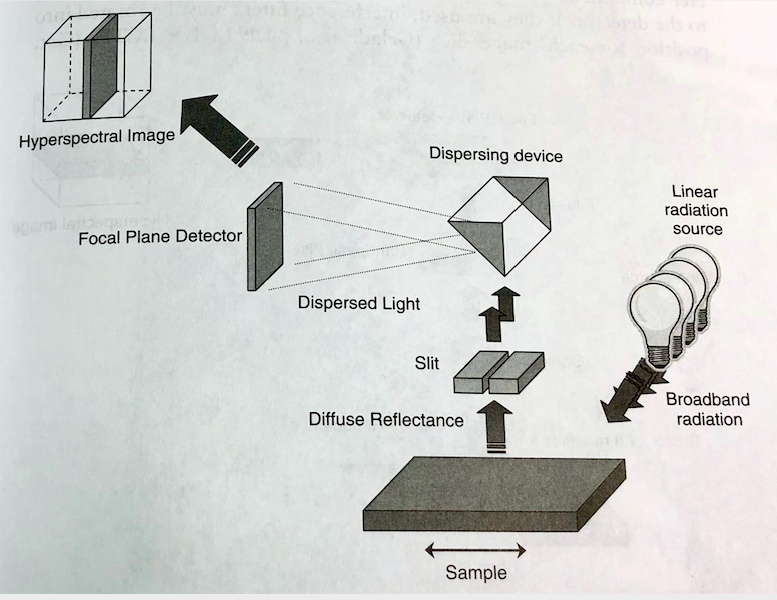
\includegraphics[height=12cm]{Images/theory/linescan.png}
%   \caption{Set-up, Line Scanning Image}
%   \label{fig:linescan}
% \end{figure}

\begin{figure}[H]
\centering
  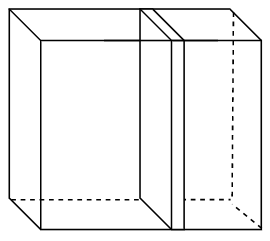
\includegraphics[height=6cm]{Images/theory/pushbroom.png}
  \caption{Resulting scan}
  \label{fig:pushbroom}
\end{figure}

\section{Georeferencing}

%http://www.gisresources.com/georeferencing-2/
In raster system, points are represented by single cells, lines by sequence of neighboring cells and area by collection of continuous cells

%http://desktop.arcgis.com/en/arcmap/10.3/manage-data/raster-and-images/fundamentals-for-georeferencing-a-raster-dataset.htm
Georeferencing means to relate an internal coordinate system to a spatial coordinate system. The internal coordinate system could for instance be a raster image of a map. 

%http://www.gisresources.com/georeferencing-2/
Note that raster systems represents points by single cells and lines by several neighboring cells. Areas are represented by a collection of continuous cells. 

In order to georeference an image, control points need to be established. These control points are identified as a series of known x- and y-coordinates, linking locations in the raster dataset to its correspondant location in the spatially referenced data. The desired objective is to assign these coordinate systems to each other with minimal residuals. This means that the distance between the control points’ actual coordinates and the coordinates predicted by the model is the smallest is can be, making the process as accurate as possible. This way, georeferencing can explain how data, such as GPS points, are related to images.


\section{SINTEF SilCam}
%https://github.com/emlynjdavies/PySilCam/wiki 
The silhouette camera, SINTEF SilCam, is a holographic imager designed to overcome the limitations in depth-of-field scenarios related to restricted path length, which is a challenge when using today's conventional lens-based imaging. 

In order to reduce noise, each image is corrected using a clean background. From this, it is possible to produce a logical image of the particles detected, containing only zeros and ones. In turn, particle properties for each particle can be calculated from the binary image.

This way, the system can be used for both large- and small-scale experiments. In smaller scale, the SilCam is able to quantify the distribution of suspended material. Zoo-plankton, larger phyto-plankton, mineral grains and marine snow are all examples of objects the SilCam can detect. 


\section{Microplastic}
%ha med hva def av mikroplast og de ulike plasttypene
%Kjemi
\todo[inline]{ta med figur av alles struktur?}
As mentioned, plastics have permeated almost every aspect of modern day life with its large applicability. We find plastics in the microchips in our computers, as well as in the bags we carry our groceries in. It seems that plastic covers a wide spectrum of applications.  One reason to this, is the many different types of plastic, covering different areas of need. Polyethylene (PE), polypropylene (PP), polyethylene terephthalate (PET), polyvinyl chloride (PVC) and polystyrene (PS), are the five most common types of plastic, in large part covering of the global plastic production. Besides containing Carbon-Hydrogen bindings, these are all structurally different and they are classified according to their chemical structure. In this section, these five types of plastic are presented in decreasing order. 

%Plastic polymers commonly found in the environment are polypropylene (PP), polyethylene (PE), polyethylene terephthalate (PET), polystyrene (PS) and polyvinylchloride (PVC).8 Together these comprise 72.9 percent of the plastic produced globally.9

\subsection{Polyethylene}
The molecules in polyethylene (PE) has the chemical formula $C_2H_4$ \todo{figur av struktur}. Polyethylene is the most common type of plastic, with 34\% of all plastic produced being PE. The reason to its commonness is the broad application of it in consumer products. Plastic bags, bottles and food wrapping are good examples of polyethylene. However, these three products seem to have a significantly different material. For instance are plastic bags rarely as rigid and as bottles. This variation in polyethylene creates two sub-types defined by the degree of density – HDPE and LDPE, high-density polyethylene and low-density polyethylene respectively. 

The LPDE-molecules are more branched, meaning that a chain is replacing for instance a hydrogen atom. As a result of this, the molecules are less tightly packed, leading to a lower density.  As LDPE has more branching than HDPE, its intermolecular forces are weaker. \todo{FIGUR av branch-forskjellene!}


\subsection{Polypropylene}
Polypropylene (PP) is the second most common plastic consistent of propylene with the chemical formula $C_3H_6$. PP has properties similar to polyethylene, but it is slightly harder and more resistant to fatigue. The plastic type is found in a variety of products like food packaging, labeling and clothing. 

\subsection{Polyvinyl Chloride}
%http://www.plasticmoulding.ca/polymers/pvc.htm
Polyvinyl chloride (PVC) with a number of vinyl chloride molecules formulated by $C_2H_3Cl$, is in third place of the most produced types of plastic. PVC can be both rigid and flexible. The rigid form is used in constructional application in piping and electrical wire insulation, while the softer and more flexible form is used in many applications replacing rubber. 

\subsection{Polyethylene terephthalate}
Polyethylene terephthalate (PET) consist of repeating ethylene terephthalate molecules, holding the chemical formula $C_{10}H_8O_4$. Typically PET is used in plastic bottles and in fibers for clothing. For the latter use, the type is commonly known as polyester. Depending on the specific particle's size and crystal structure, the semi crystalline material, PET, might appear transparent. 

\subsection{Polystyrene (PS)}
%https://www.azom.com/article.aspx?ArticleID=7915
Polystyrene (PS) is an inexpensive plastic type commonly used for packaging purposes, with the chemical formula being $(C_8H_8)_n$. PS increasingly exists in the outdoor environment, particularly along shores. The plastic is naturally clear, hard and brittle. The latter fact is perhaps the main reason to why larger pieces of PS easily turn into microplastic. 



\section{Principal Component Analysis}

The purpose of conducting a principal component analysis is to extract the information from the data, while disregarding the noise, reducing the dimension of the dataset. The analysis converts a set of observations of possibly correlated variables into a set of values of linearly uncorrelated variables called principal components. These principal components will describe the overall variation of the dataset and thereby serve as a latent variable. 
\\\\
Now, how are these principal components found? Figure a) below describes the entire dataset with the dots describing single data observations. The analysis starts by finding the projection of each observation onto a line. The line is drawn with the purpose of explaining as many observations as possible with a minimal residual error, b). The distance from the origin to this projected point along the line is the score associated with the related observation. The direction of the line is now characterized with giving the largest variance of the scores, and is described by direction vectors called loadings. 
\\\\
%Simply put, the original data is estimated by multiplying the scores with the associated loadings.
This first line created is called the first principal component. The second principal component, c), is perpendicular to the first component’s direction and is otherwise found the same way. This way, the first principal component has the largest possible variance. Each following component will, in turn, have the highest variance possible under the constraint that it is perpendicular to the previous components. 

%FIGURENE:
%https://learnche.org/pid/latent-variable-modelling/principal-component-analysis/geometric-explanation-of-pca
\begin{figure}[H]
  \newcommand*\FigVSkip{0.5em}
  \newcommand*\FigHSkip{0.1em}
  \newsavebox\FigBox
  \centering
  % Top image is centered, so no need to get width
\sbox{\FigBox}{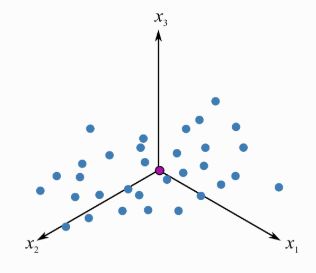
\includegraphics[scale=0.4]{Images/theory/koord.png}}
  \begin{minipage}{\wd\FigBox}
    \centering\usebox{\FigBox}
    \subcaption{a) Scaled and centered data observations}
  \end{minipage}
 \sbox{\FigBox}{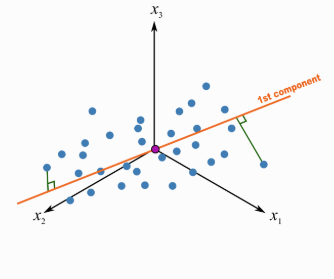
\includegraphics[scale=0.4]{Images/theory/1pc.png}}
  \begin{minipage}{\wd\FigBox}
    \centering\usebox{\FigBox}
    \subcaption{\newline b) Including first principal component}
  \end{minipage}
  % Save first image in a box to get the width
  \sbox{\FigBox}{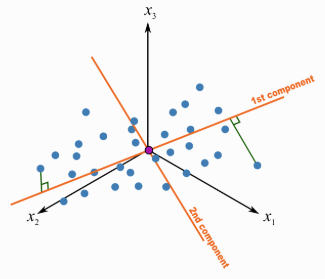
\includegraphics[scale=0.4]{Images/theory/2pc.png}}
  \begin{minipage}{\wd\FigBox}
    \centering\usebox{\FigBox}
    \subcaption{c) Including second principal component}
  \end{minipage}\hspace*{\FigHSkip}
  % Save second image 
  \label{head}
\end{figure}



\todo[inline]{Skrive om den under til både forsøksrelevant og ny}
%Underwater hyperspectral imaging: a new tool for marine archaeology 2018, ØYVIND ØDEGÅRD,1,2,* AKSEL ALSTAD MOGSTAD,3 GEIR JOHNSEN,3 ASGEIR J. SØRENSEN, AND MARTIN LUDVIGSEN1
To assess the spectral relationship between different objects and materials, principal component analyses were performed on the laboratory-acquired reflectance data. The principal components can be seen as the axes in an ellipsoid with n dimensions that describes the data. The longest axis accounts for the largest variance in the data, and corresponds to principal component 1 (PC1). The second-longest axis corresponds to PC2, and so on.

\subsection{Scores, Loadings, F-residuals, Hotellings T^2 }
https://learnche.org/pid/latent-variable-modelling/principal-component-analysis/interpreting-the-residuals

\section{Sensor Carrying Platform}
%ulike sensorer for deteksjon og kartlegging (vise sammenhengen til dette og en bredere oversikt - dette blir isåfall bare her, men tas ikke med videre - i metode kan vi heller si at vi avgrenser mot cam. + aktuelle sensorer







%\subsection{General behavior changes in water}
%\subsection{Lysets oppførsel i vann}

\chapter{{Approach/Method}}
\section{Hyperspectral Imaging} 
%evt bare spektrometeret - teste alle de ulike typene plast som vi har kjøpt fra tyskland 


\subsection{Purpose}
The purpose of the experiment is to get a better understanding of the properties of specific plastic types. By looking at how light is reflected from different types of plastic, it will be possible to compare the plastic types and hopefully detect some kind of pattern. Initially, the plastic pellets will be examined in a dry environment, before being placed in water later on. These results will be compared in order to see if experiments carried out in dry environment can be representative for plastic pellets in wet environment. 

\subsection{Hypotheses}
$\bullet$ Different types of plastic provide different signatures in the visible light spectrum\\ 
$\bullet$ Various types of plastic provide different signatures in infrared light spectrum\\
$\bullet$ Different types of plastic have different intensities of reflecting light\\
$\bullet$ Varying thickness in a specific type of plastic, will give different results\\
$\bullet$ Post consumer recycled pellets and clean pellets have different signatures\\
%Hvis dette stemmer, må vi finne ut om plasten noen gang kan anses som ”clean” i livsløpet (for eksempel på starten/etter hvert som farge osv er vasket av)
$\bullet$ The same type of plastic gives a similar signature in water as well as in a dry environment

\subsection{Material}
\begin{center}
\Rotatebox{0}{
\begin{tabular}{ |c|c|c|c|c| }
 \hline
 \textbf{Ref Number} & \textbf{State} & \textbf{Class} & \textbf{Additives} \\ 
 
 CRT131.00 & Post-Industrial Recyclate Pellets & PE: LDPE/LLDPE & Yes, colorants\\
 CRT150.00 & Post-Consumer Recyclate Regrind & PE-HD & Colorants \\
CRT170.00 & Environmental Pellets & PE: LDPE/HDPE & Yes \\
CRT171.00 & Environmental Fragments (Regrind) & PE-HD & Yes \\
CRT200.00 & Pristine Pellets & PP-Homopolymer & Yes, stabilizers \\
CRT250.00 & Post Consumer Recyclate: Pellets & PP Mixture & Yes \\
CRT300.00 & Pristine Pellets & PS General purpose & Unknown \\
CRT331.00 & Post Consumer Recyclate Regrind & PS Mixture & Yes \\
CRT400.00 & Pristine Pellets & PET Amorphous & No, not intentionally \\
CRT451.00 & Post Consumer Recyclate Regrind & PET Amorphous & No, not intentionally \\
CRT500.00 & Pellets & PVC Soft & Yes, softener \\
CRT530.00 & Pellets & PVC Hard & Yes, softener \\
 \hline
\end{tabular}
}
\end{center}
%$\bullet$ plastpose\\\\
%$\bullet$ plastflaske\\\\
%$\bullet$ …?

\subsection{Equipment} 
(from ocean optics web page)\\
$\bullet$ QE Pro spectrometer - measures optical signatures on the specific object. In this experiment, reflectance is used to illustrate the color properties\\
$\bullet$ WS-1 Reflectance Standards - 100 percent reflectance within 250-1500 nanometers\\
$\bullet$ QR400-7-VIS-BX reflection probe, light out and reflectance in\\
$\bullet$ RPH reflective probe holder, holding the reflection probe in a 45 degree angle and keeping the source 1 cm away from the measured object\\
$\bullet$ OceanView 1.6.7 - The program used to visualize the object reflectance \\
$\bullet$ Light source

\subsection{Procedure} 
The spectrometer is turned on and connected to OceanView 1.6.7 via an external computer. In OceanView, the spectrometer is set to a constant temperature of -10 degrees (Celsius). The QR400-7-VIS-BX reflection probe is connected to the spectrometer through one cable, and a light source through another. In addition, the reflection probe is placed in a reflective probe holder, angling the light output (and the sensor inlet) in order to avoid specular reflection. This angle is set to 45 degrees.
\\\\
Furthermore, the reflective probe is placed over the object to be measured. To begin with, this is the WS-1 Reflectance Standards with 100 percent reflectance within the range of 250-1500 nanometers. This is measured in OceanView and sets the standard for white. Furthermore, the reflective probe holder is placed over the specific plastic type to be measured. The reflectance from the plastic pieces is then visualized in OceanView and is ready for comparison. This process will be repeated with different types of plastic.
\\\\
%Underwater hyperspectral imaging: a new tool for marine archaeology 2018, ØYVIND ØDEGÅRD,1,2,* AKSEL ALSTAD MOGSTAD,3 GEIR JOHNSEN,3 ASGEIR J. SØRENSEN, AND MARTIN LUDVIGSEN1
We assume ideal lighting such that the measured radiance of an object is independent of its position on the scan line. Additionally, the reference plate is assumed to reflect the downwelling radiance equally at all wave- lengths. 

%Samme gjennomføres i vann?
%Samme gjennomføres med store plastbiter?

%Ønsket resultat?

\section{Underwater Hyperspectral Imaging} 

\section{Introducing a SilCam Lens} Implementere linsen i tidligere oppsett. 

\section{PCA} Denne baseres på dataen funnet fra metodene over: finner ut hvor sensitiv plasttypen er for forskjellige bølgelengder - er dette en plasttype som gir samme signatur over alle bølgelengder og er uniform feks?

\subsection{Classification} Herunder klassifisering og kategorisering - feks basert på signatur. (Leter etter en trender i datasettet.)

\section{Measurement of Success}
Målestokk for suksess

\chapter{Results}
%Merk at vi egentlig mener at diskusjonen i seg selv er en del av resultatet! Bruk diskursjon som et underpunkt til resultat
\section{Results from the Spectrometer I} 
the wave spectrum from one of the types. This can be compared to the associated colors wave spectrum. 
\section{Results from the Spectrometer II}
Comparing the signature of two different types of plastic (de gjennomsiktige pelletsene), which more or less have the same signature
\section{Principal Component Analysis I}
Using the different types of plastic only

\section{Principal Component Analysis II} 


\section{The Final Method} 

\chapter{Discussion}
Klassifisering basert på PCA-resultatene





VISUAL LIGHT
Experiments analyzing the wave spectra of different types of plastics, have already been conducted. However, the results has been directed towards viewing the wave length interval describing near infrared light (NIR). Although the use of infrared light is an effective means of unobtrusive observation on land, it is far less effective in the ocean because long wavelength light is rapidly attenuated by seawater.

%https://oceanoptics.com/plastic-recycling-nir-spectroscopy/
Another important observation in these experiments, is the condition of the microplastic used. The material is pure and white, making the results independent of color. 

Water absorption 
%https://commons.wikimedia.org/wiki/File:Absorption_spectrum_of_liquid_water.png
This logarithmic (log-log) graph shows water’s absorption behavior at different colors wavelength. As seen in the graph, water absorption is minimized between 400 -600 nm


Light Transmission in the Ocean: http://www.waterencyclopedia.com/La-Mi/Light-Transmission-in-the-Ocean.html
https://manoa.hawaii.edu/exploringourfluidearth/physical/ocean-depths/light-ocean


AN IDEA:
In order to obtain a color-free spectrum, one could subtract the color spectrum from the resulting spectrum retrieved from the experiments. However, most pieces of plastic do not have one specific color, making it difficult to determine the spectrum to subtract. 

In addition. When experimenting with different types of plastics having more or less the same colors, the results turned out next to identical. At first, a thought was that this was due to the color being too dominant in relation to the rest of the properties. However, conducting the same experiment with non-colored pieces of plastic, gave the same end-result; no difference in spectral signature even if the types of plastics differ. - this could also be due to reflectance disturbance from "shiny" see through material. 

ANOTHER IDEA: 
What if we could inspect the level of additive acceptance in the different types of plastic. By finding the most resistant types, it might be possible to modify these into doing the same job as the types accepting additives. This way, we could reduce the production of the largest vectors/toxin-carriers. 

\chapter{Conclusion and Recommendation for Further Work}
Husk å ikke være for skråsikre - ikke lukk en dør før vi er HELT sikre!
Besvare spm i introduksjonen!

\section{Further Work}
Her kan jeg plukke opp trådene fra teoridelen som tar for seg sensorer og sensorbærende platformer. Snakke om hvordan deteksjonsmåten vi har funnet nå, kan implementeres på et fartøy og utnyttes.


\appendix
\chapter{Chapter 1 of appendix}
Appendix chapter 1 text goes here

\bibliography{sampleThesis}

\end{document}